\section{Survey}
%Context about why we needed the data

%How the whole thing went down
In order to make a dataset in a short time frame, we looked into crowdsourcing, where it was possible to pay people to answer surveys or do tasks that computers cannot. In particular we were looking at Clickworker and Mechanical Turk, which allowed external surveys. Since no sites had an inbuilt survey creation tool that could handle our requirements, we decided to make our own survey website.

Using this method, we could potentially reach thousands of people without limiting us to the survey tools made available on the standard websites.

%Creation of the website
For web hosting, we went to DigitalOcean, which offered a Ubuntu server setup with Django. We added Gunicorn as the WSG interface and nginx as the http server. Behind it all, we had a MySql database keeping track of the survey questions and results along with timestamps.

%Django as Python web application framework
%Gunicorn as Web Server Gateway Interface(WSGI) server. A traditional web server does not understand or have any way to run Python applications. WSGI is a standard interface for py modules and containers.
%Digical Ocean as webhost with Unix as the OS
%MySql as the database

%The survey
The survey itself asks participants to personally give a recommendation to a group of users. The participant knows each user's own top 10 preference, and must decide on their own what aggregation strategy they wish to follow. An important aspect of the survey was making it as easy to complete as possible. As we had to pay each participant, each such improvement could be translated to a saving, which in turn translated to a larger and more useful dataset. So to make it more intuitive and not overload each user with information, we made it so that hovering the mouse over a movie title will make the movie's position light up on all the other users' rankings, shown in Figure \ref{fig:appendix_userprefs}, and gave the user a tooltip about other movie positions. Additionally, we made the ranking system into a drag-and-drop, such that the participant could drag and easily rearrange their recommendations. This can be seen in Figure \ref{fig:appendix_recbox}.

\begin{figure}\label{fig:appendix_recbox}
	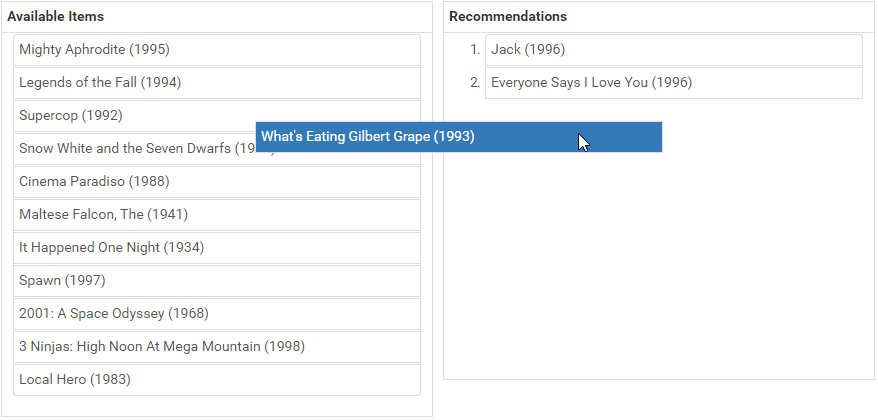
\includegraphics[scale=0.35]{graphics/recbox.png}
	\caption{The list of available items and the box holding the recommendations of the survey participant}
\end{figure}

\begin{figure}\label{fig:appendix_userprefs}
	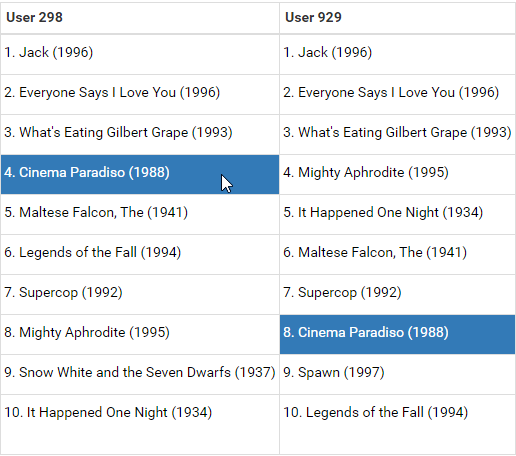
\includegraphics[scale=0.5]{graphics/users.png}
	\caption{Two lists of movie preferences for a user}
\end{figure}

After making a recommendation, the user could proceed to the next step, and upon completing all steps they would reach a screen providing them with a code. With each step, the group size is increased by one, going from 4 to 8 users. The code is important, as the participant must present this as evidence to the crowdsourcing site as proof of their participation. For our survey, we decided to generate a unique code for each participant mixing the assigned groups and a timestamp, so that we could deduce which user responded when and with what. This precaution was necessary so that it was possible to filter out participants rushing through the survey with no care for their answers.

Also, since we wanted to have a balanced dataset, we separated our groups into 40 sets of groups of size 4 to 8, and made it so that every user would get a randomly picked set. The database would keep track of how many responses each set had, such that we could prioritize the sets with fewer responses and get a balanced dataset. It would also mean that anyone taking the test twice would be unlikely to see the same survey.

Before running the survey on Mechanical Turk, we ran it past some other willing participants for evaluation and decided to halve the number of groups each participants would give recommendations to from 10 to 5, due to feedback about the length of the survey. \note{This section can be expanded to better reflect the process and changes happening to the survey, as a lot of work went into it in the project}

%Most importantly, we realized how vital it was to make the par

%Dealing with mechanical turk
For the crowdsourcing website, we ended up going with Amazon's Mechanical Turk, as it is the more well-known and cheaper service. When ready, we injected a good amount of money on the account, as one had to prepay for any work requested and started up a limited run to test out the services and find a suitable price range. We managed to get a few responses. On Mechanical Turk, the participant would see our survey, click in and be provided a link to our survey. Upon completion of the survey, our participant would get the code and input it on the Mechanical Turk website. Initial results were interesting with big differences between how much time participants spent on the survey. We noted a few obvious cheaters who blazed through a survey in seconds thanks to the timestamps, however as a requester and with the timestamps in our database, we would be able to sort them out, and we could also reject their work on the Mechanical Turk site.

Though, on the third day of this limited run we ran into problems with Amazon Mechanical Turk. We were unable to access our account, and had to contact their support team. Soon enough the support team responded that our account had been suspended, and that we would be informed about the reason for the suspension in 2-3 days along with fate of our account. In two days time, Mechanical Turk support wrote us that our account had been suspended indefinitely and our current survey stopped because of a violation of the participation agreement. Unaware of any possible violations we could have made, we made further inquires, but never got a clear answer. Additionally, our funds on the account were also confiscated. So in the end, we ended up only getting responses totaling a few dollars worth of data.

%Show data and evaluate on them.